\documentclass[10pt,letterpaper,twocolumn]{article}

% Compact two-column research-paper typography.
\usepackage[T1]{fontenc}
\usepackage{newtxtext,newtxmath}
\usepackage[letterpaper,top=0.64in,bottom=0.70in,left=0.68in,right=0.68in,
            headheight=11pt,headsep=0.12in,footskip=0.26in]{geometry}
\usepackage[protrusion=true,expansion=true]{microtype}
\usepackage{amsmath}
\usepackage{graphicx}
\usepackage{xcolor}
\usepackage{titlesec}
\usepackage{fancyhdr}
\usepackage{enumitem}
\usepackage{placeins}
\usepackage{dblfloatfix}
\usepackage{balance}
\usepackage[font=footnotesize,labelfont=normalfont,labelsep=period,
            justification=justified,singlelinecheck=false]{caption}
\usepackage[numbers,sort&compress]{natbib}
\usepackage[hidelinks]{hyperref}
\urlstyle{same}
\hypersetup{
  pdftitle={Shared Information Sources in Epistemic Networks},
  pdfauthor={Rohan Goyal}
}

% Page and paragraph geometry
\setlength{\columnsep}{0.27in}
\setlength{\columnseprule}{0pt}
\setlength{\parindent}{1.05em}
\setlength{\parskip}{0pt}
\setlength{\emergencystretch}{2em}
\setlength{\bibsep}{0pt}
\setlist{topsep=0.35em,itemsep=0.08em,parsep=0pt,partopsep=0pt,leftmargin=*}
\raggedbottom
\setcounter{topnumber}{2}
\setcounter{bottomnumber}{2}
\setcounter{totalnumber}{4}
\setcounter{dbltopnumber}{1}
\renewcommand{\topfraction}{0.90}
\renewcommand{\bottomfraction}{0.78}
\renewcommand{\textfraction}{0.10}
\renewcommand{\floatpagefraction}{0.82}
\renewcommand{\dbltopfraction}{0.88}
\renewcommand{\dblfloatpagefraction}{0.82}
\makeatletter
\setlength{\@fptop}{0pt}
\setlength{\@fpsep}{8pt plus 2fil}
\setlength{\@fpbot}{0pt plus 1fil}
\makeatother

\renewcommand{\thesection}{\Roman{section}}
\renewcommand{\thesubsection}{\Alph{subsection}}
\titleformat{\section}[block]
  {\centering\normalfont\fontsize{9.2}{10.8}\selectfont\bfseries}
  {\thesection.}{0.55em}{\MakeUppercase}
\titlespacing*{\section}{0pt}{2.0ex plus 0.35ex minus 0.2ex}{0.85ex}

\titleformat{\subsection}[block]
  {\normalfont\fontsize{8.8}{10.2}\selectfont\itshape}
  {\thesubsection.}{0.50em}{}
\titlespacing*{\subsection}{0pt}{1.45ex plus 0.25ex minus 0.15ex}{0.45ex}

\titleformat{\paragraph}[runin]
  {\normalfont\fontsize{8.7}{10.1}\selectfont\bfseries\itshape}
  {}{0pt}{}
\titlespacing*{\paragraph}{0pt}{1.0ex plus 0.2ex minus 0.1ex}{0.45em}

\pagestyle{fancy}
\fancyhf{}
\fancyhead[R]{\fontsize{8}{9}\selectfont\thepage}
\renewcommand{\headrulewidth}{0pt}
\renewcommand{\footrulewidth}{0pt}
\fancypagestyle{firstpage}{%
  \fancyhf{}
  \fancyhead[R]{\fontsize{8}{9}\selectfont\thepage}
  \renewcommand{\headrulewidth}{0pt}
}

\renewcommand{\figurename}{FIG.}
\captionsetup{belowskip=0pt,aboveskip=4pt}

\newcommand{\makepapertitle}{%
  \thispagestyle{firstpage}%
  \begin{center}
    \vspace*{-0.22in}
    {\fontsize{14.2}{16.2}\selectfont Shared Information Sources in Epistemic Networks\par}
    \vspace{0.78em}
    {\fontsize{10.2}{11.8}\selectfont Rohan Goyal\par}
    \vspace{0.18em}
    {\fontsize{8.4}{9.8}\selectfont (Draft: \today)\par}
  \end{center}
  \vspace{0.48em}
}

\newenvironment{paperabstract}
  {\begin{center}\begin{minipage}{0.72\textwidth}
   \fontsize{9.0}{10.6}\selectfont\noindent}
  {\end{minipage}\end{center}\vspace{0.72em}}

\begin{document}
\twocolumn[
\begin{@twocolumnfalse}
\makepapertitle
\begin{paperabstract}
\noindent
We study how a common external information source affects collective learning in
an epistemic-network model. Bayesian agents choose between a safe action with a
known success rate and an experimental action with an unknown but higher success
rate. Agents update from their own trials and from evidence shared by network
neighbors. We add a source consulted by a fixed fraction of agents and vary the
source's signal accuracy, influence, adoption, updating rule, and within-round
signal dependence. A static source emits signals with fixed accuracy. An
adaptive source updates from the community's experimental data. In the
parameter settings examined, four patterns recur. First, independent signals of
equal marginal accuracy often yield higher correct-consensus rates than a common
signal (a \emph{correlation penalty}), especially when the problem is difficult
and agents place substantial weight on the source. Second, a shared biased source
can leave a networked community worse off than the same community without the
source, and in some regimes worse off than a lone agent facing the same source.
Third, an adaptive source that learns from community data performs close to the
no-source baseline and far below a static source of fixed high accuracy; in
incorrect adaptive runs, experimentation on the better action ceases and the
source's posterior stops changing. Fourth, complete and cycle networks reverse
their relative ranking as source accuracy changes. Adaptive trust updating
provides only limited protection against biased sources and can reduce the gains
from reliable ones. These simulation results do not establish a general ordering
of network structures or a direct policy prescription. They show that the effects
of a shared source depend jointly on signal correlation, endogenous evidence
production, trust adjustment, and social network topology.
\end{paperabstract}
\end{@twocolumnfalse}
]

\section{Introduction}
\label{sec:intro}

Communities increasingly use common algorithmic systems to search, summarize,
rank, and evaluate information. When many users rely on the same system, its
outputs can correlate their judgments and actions. This raises a question about
collective learning: how does a common external source affect a community whose
members also gather evidence and communicate with one another?

Several existing literatures address parts of this question. Models of
algorithmic monoculture show that common decision rules or common information
can homogenize outcomes and reduce aggregate performance even when the shared
system is useful to an individual decision maker \citep{kleinberg2021,
bommasani2022}. Work on social learning and multi-armed bandits shows that
myopic agents can collectively under-explore superior options
\citep{banihashem2023}. Most directly, \citet{heddenraghavan2026} compare
monoculture and polyculture in a bandit setting and show that independent
information groups can preserve exploration that is lost when all agents share
the same history of actions and rewards.

This study examines how such effects interact with communication topology. The
model separates the network through which agents exchange experimental evidence
from the dependence structure of advice supplied by an external source. Agents
remain embedded in a Zollman-style epistemic network
\citep{zollman2007,zollman2010}, while source signals can reach adopters
independently of the network edges. This design allows several comparisons:
common versus independent source signals at fixed marginal accuracy; the same
source in different communication networks; a static source versus an adaptive
source that learns from community-generated evidence; a networked community
versus a lone agent facing the same source; and fixed versus endogenously
updated trust in the source.

The simulations yield four principal results, together with a secondary finding
on adaptive trust. First, across several parameter combinations, common signals
produce lower correct-consensus rates than independent signals of the same
marginal accuracy---a \emph{correlation penalty}. Second, individual and
collective consequences of the same source can diverge: under a shared biased
source, a cycle network can fall well below its no-source baseline and below a
lone agent consulting the same source. Third, under an adaptive source that
updates from community data, correct-consensus rates remain close to the
no-source baseline and far below those obtained with a static source of fixed
high accuracy; incorrect adaptive runs enter a state in which agents stop
testing the better action and the source therefore receives no revising
evidence. This mechanism is related to decision-dependent data generation in
performative prediction \citep{perdomo2020}. Fourth, the complete and cycle
networks reverse their relative ranking as source accuracy changes. Adaptive
trust updating, examined as a remedial mechanism, improves outcomes modestly
under some biased-source conditions on the cycle but can reduce the benefit of
reliable sources on the complete graph.

The study contributes a model in which the dependence structure of external
advice varies independently of the network structure of social learning. Its
claims are confined to the simulated mechanisms and parameter regions examined,
consistent with evidence that results in this model family are
parameter-sensitive \citep{rosenstock2017}.

Section~\ref{sec:related} reviews the closest work. Section~\ref{sec:model}
specifies the model and simulation protocol. Sections~\ref{sec:baseline}--
\ref{sec:trust} report the baseline, static-source, adaptive-source, and
adaptive-trust results. Section~\ref{sec:discussion} discusses interpretation,
limitations, and directions for further tests.

\section{Related Work}
\label{sec:related}

\subsection{Network epistemology}

Building on Bayesian learning models in economics \citep{balagoyal1998}, the
models developed by \citet{zollman2007,zollman2010} represent agents who choose
between actions, observe outcomes, and exchange evidence over a social network.
Because agents stop collecting evidence about an action they no longer choose,
early unfavorable samples can cause a community to abandon the superior action.
Sparse networks can sometimes outperform complete networks by preserving
heterogeneity in behavior long enough for additional evidence to be generated.
This is commonly described as the epistemic benefit of transient diversity.

The comparative performance of sparse and dense networks is parameter-dependent.
\citet{rosenstock2017} show that network rankings change across model settings
and caution against general policy conclusions from a limited set of simulations.
Subsequent work has examined biased agents, propaganda, and selective trust
within epistemic networks \citep{weatherall2020,oconnor2019}. The model developed
here adds an external source whose signals need not travel along the social
network, allowing signal correlation to vary independently of network
connectivity.

\subsection{Algorithmic monoculture and collective exploration}

\citet{kleinberg2021} show that adoption of a common algorithm can reduce social
welfare by correlating decisions, even when the algorithm is more accurate for
an individual user. \citet{bommasani2022} study outcome homogenization when
systems share data or models. These studies concern selection outcomes rather
than repeated truth-directed learning, but they establish the general point that
individual accuracy does not determine system-level performance.

The closest comparison is the bandit analysis of
\citet{heddenraghavan2026}. Their monoculture condition gives sequential agents
a common history of previous actions and rewards, whereas their polyculture
condition partitions agents into independent information groups. They show that
polyculture can be more likely to identify the best arm because each information
group has an independent chance to continue exploring it. Related work in
computer science establishes learning failures among myopic agents who observe
prior bandit outcomes \citep{banihashem2023}.

In the model developed here, all agents retain the same social evidence-sharing
structure across source conditions. The experimental comparison varies whether
external advice is common or independently drawn while holding the social
network fixed. Source correlation and network topology can therefore be analyzed
separately. A separate lone-agent benchmark isolates private consequences of the
same source from networked collective outcomes.

\subsection{Feedback from decisions to data}

The adaptive-source condition is related to performative prediction, in which a
prediction changes behavior and thereby changes the distribution of later data
\citep{perdomo2020}. It is also related to feedback in recommender and
decision-support systems. Here, the relevant feedback concerns whether
source-influenced experimentation continues to generate evidence capable of
revising the source's posterior.

\section{Model and Simulation Protocol}
\label{sec:model}

\subsection{Agents, actions, and priors}
\label{sec:agents}

A community of $N$ agents repeatedly chooses between two Bernoulli actions. The
safe action $a$ has a known success probability $p_s=0.5$. The experimental
action $b$ has unknown success probability
\begin{equation}
  p_b = p_s + \varepsilon, \qquad \varepsilon>0,
\end{equation}
so $b$ is objectively better. Agent $i$ represents uncertainty about $p_b$ with
a Beta distribution,
\begin{equation}
  \theta_i\sim\mathrm{Beta}(\alpha_i,\beta_i), \qquad
  \mu_i=\frac{\alpha_i}{\alpha_i+\beta_i}.
\end{equation}
At initialization, each agent draws a prior mean
$\mu_i(0)\sim\mathrm{Uniform}(0,1)$ and receives prior concentration $c$:
\begin{equation}
  \alpha_i(0)=c\mu_i(0), \qquad
  \beta_i(0)=c[1-\mu_i(0)].
\end{equation}
The heterogeneous prior means ensure that some runs begin with agents willing
to test $b$. If every agent initially preferred the known safe action and agents
never explored, no evidence about $b$ would be produced.

\subsection{Action choice and evidence sharing}
\label{sec:sharing}

At the start of round $t$, agent $i$ chooses $b$ if $\mu_i(t)>p_s$ and chooses
$a$ otherwise. An agent choosing $b$ conducts $m$ trials and observes
$k_i\sim\mathrm{Binomial}(m,p_b)$ successes. Trials of $a$ provide no information
about $p_b$ because $p_s$ is known.

Let $G$ be the undirected communication graph and let $\mathcal{N}^{+}(i)$
include agent $i$ and its neighbors. After experimentation, agent $i$ updates on
all $b$-trials generated in $\mathcal{N}^{+}(i)$:
\begin{align}
  \alpha_i &\leftarrow \alpha_i+
  \sum_{\substack{j\in\mathcal{N}^{+}(i)\\j\text{ chose }b}} k_j,\\
  \beta_i &\leftarrow \beta_i+
  \sum_{\substack{j\in\mathcal{N}^{+}(i)\\j\text{ chose }b}}(m-k_j).
\end{align}
Agents exchange trial outcomes, not posterior means. We examine complete, cycle,
wheel, Erd\H{o}s--R\'enyi, small-world, and scale-free graphs where noted. Unless
otherwise stated, Erd\H{o}s--R\'enyi graphs use edge probability $0.3$
(conditioned on connectivity), Watts--Strogatz graphs use ring degree $k=4$ and
rewiring probability $0.1$, and Barab\'asi--Albert graphs use attachment
parameter $m=2$. The main source comparisons use the complete and cycle graphs.

\subsection{External source}
\label{sec:source}

At the start of each run, a fixed fraction $\varphi$ of agents is designated as
source adopters by uniform random selection without regard to network position.
In each round, an adopter consults with probability $q$. Consultation adds
$\tau$ pseudo-observations to the agent's Beta parameters. If the source
communicates an implied success rate $v_i\in(0,1)$, then
\begin{equation}
  \alpha_i\leftarrow\alpha_i+\tau v_i, \qquad
  \beta_i\leftarrow\beta_i+\tau(1-v_i).
  \label{eq:source}
\end{equation}
The parameter $\tau$ controls the source's influence on posterior belief. Because
source information is incorporated after action choice and experimental updating
in a round, it affects the agent's choice in the following round.

\paragraph{Static source.}
The static source has fixed signal accuracy $r$. In each round it favors the
better action $b$ with probability $r$ and favors $a$ otherwise. An endorsement
of $b$ is encoded as $v=h$; an endorsement of $a$ is encoded as $v=1-h$, where
$h\in(0.5,1)$ controls signal strength. In the \emph{common-signal} condition,
all adopters who consult in the same round receive the same draw. In the
\emph{independent-signal} condition, each consulter receives a separate draw with
the same accuracy $r$. Thus the two conditions have the same marginal signal
distribution and differ in within-round dependence.

The source is static in the sense that its accuracy and signal-generation rule
remain fixed throughout a run.

\paragraph{Adaptive source.}
The adaptive source maintains a Beta posterior
$\mathrm{Beta}(\alpha_O,\beta_O)$ over $p_b$, initialized as
$\mathrm{Beta}(1,1)$, and communicates its current posterior mean
\begin{equation}
  v=\mu_O=\frac{\alpha_O}{\alpha_O+\beta_O}.
\end{equation}
After agents have acted and consulted, the source updates on all $b$-trials
produced by the community in that round:
\begin{align}
  \alpha_O&\leftarrow\alpha_O+
  \sum_{j:j\text{ chose }b}k_j,\\
  \beta_O&\leftarrow\beta_O+
  \sum_{j:j\text{ chose }b}(m-k_j).
\end{align}
If no agent chooses $b$, the source receives no new information. This condition
creates a feedback channel because the source affects later choices and those
choices determine the source's later data.

\paragraph{Adaptive trust.}
In some simulations, adopters scale the base influence $\tau$ by an exponential
moving average of agreement between the source's endorsement and the community's
realized experimental evidence in rounds where $b$ is tested. When agreement
falls below a coin flip, effective trust is reduced toward zero. This mechanism
asks whether agents can discipline a biased source by withdrawing weight from its
testimony, provided enough exploration remains to expose the bias.

\subsection{Timing}
\label{sec:timing}

Each round proceeds as follows: (1) agents choose actions from beliefs at the
start of the round; (2) agents choosing $b$ run experiments; (3) agents update
on evidence produced by themselves and their neighbors; (4) consulting adopters
incorporate source information using Eq.~\eqref{eq:source}; (5) the adaptive
source, when present, updates from all community evidence about $b$; and (6)
adaptive trust, when enabled, updates from agreement between the source and
realized evidence. The order creates a one-round lag between a source signal and
the action it influences.

\subsection{Outcomes and Monte Carlo estimation}
\label{sec:outcomes}

A run stops when all agents remain on the same side of $p_s$ for $S$ consecutive
rounds or when the horizon $T_{\max}$ is reached. At termination, a run is
classified as correct if at least a fraction $\rho$ of agents have
$\mu_i>p_s$, incorrect if at most $1-\rho$ do, and unresolved otherwise. We use
$\rho=0.99$.

The primary outcome is the estimated probability of correct consensus across
independent random seeds. Secondary outcomes are the incorrect-consensus rate,
time to termination, the fraction $f_t$ of agents choosing $b$, and the binary
entropy of action choice,
\begin{equation}
  H_t=-f_t\log_2f_t-(1-f_t)\log_2(1-f_t),
\end{equation}
with $H_t=0$ when $f_t\in\{0,1\}$. For the adaptive source, we also record
$\mu_O(t)$. Reported standard errors treat each seed as an independent Bernoulli
trial for the consensus indicator.

Unless otherwise indicated, the default parameters are
$\varepsilon=0.05$, $N=10$, $m=1$, $c=4$, $T_{\max}=800$, $S=8$,
$q=1$, $h=0.75$, and $\tau=1$. Grid estimates use $1000$ Monte Carlo seeds per
cell; the lone-agent benchmark uses $4000$ seeds; adaptive-source trajectory
bands use $300$ seeds. Source comparisons that do not vary adoption use
$\varphi=1$ unless noted. Adaptive-trust comparisons use $\varphi=0.7$,
$\tau=2$, and learning rate $0.15$.

\section{Baseline Results}
\label{sec:baseline}

We first test whether the implementation reproduces the qualitative result that
network topology can affect the probability of correct consensus in the absence
of an external source. Complete, cycle, wheel, Erd\H{o}s--R\'enyi, small-world,
and scale-free networks are compared over $\varepsilon\in\{0.02,0.05,0.10\}$ at
$N=10$.

\begin{figure*}[!t]
\centering
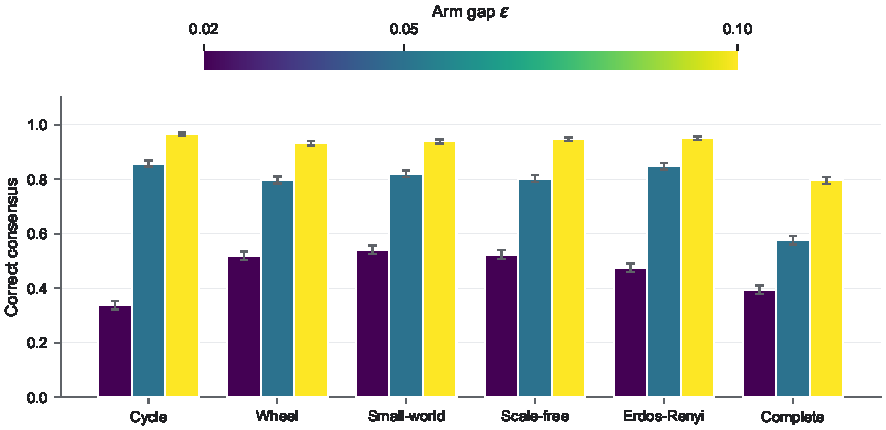
\includegraphics[width=0.80\textwidth]{figures/baseline_network_reliability.pdf}
\caption{Correct-consensus probability without an external source, by network
topology and arm-quality gap $\varepsilon$. Smaller values of $\varepsilon$
represent more difficult discrimination problems. Each bar aggregates $1000$
Monte Carlo runs at $N=10$; error bars show one standard error.}
\label{fig:baseline}
\end{figure*}

At $\varepsilon=0.05$ and $N=10$, the cycle reaches correct consensus more often
than the complete graph (approximately $0.86$ versus $0.58$). The ordering
changes at other values of $\varepsilon$: at $\varepsilon=0.02$, the cycle can
itself perform poorly relative to denser graphs. The result reproduces the
parameter-dependent transient-diversity effect reported in prior
network-epistemology models (Fig.~\ref{fig:baseline}).

\section{Static-Source Results}
\label{sec:static}

\subsection{Signal accuracy and adoption}

We vary source signal accuracy $r$, adoption fraction $\varphi$, and topology
under a common static source with $\tau=1$. Higher adoption amplifies the
effects of the source in both directions: when $r<0.5$, adoption lowers the
correct-consensus rate; when $r$ is high, adoption raises it. In the displayed
parameter region, the cycle exhibits a sharper transition across $r$ than the
complete graph (Fig.~\ref{fig:heatmaps}). The dashed contour marks the
no-source baseline for each topology. The shape and location of this transition
vary with the remaining model parameters.

\begin{figure*}[!t]
\centering
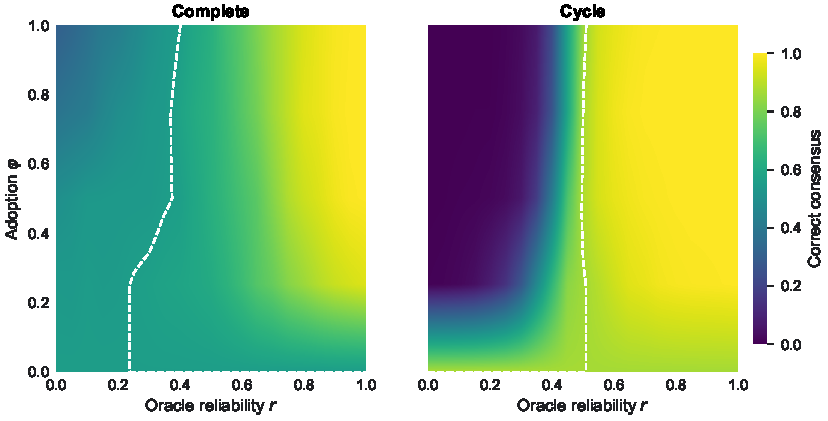
\includegraphics[width=0.86\textwidth]{figures/fixed_testimony_heatmaps.pdf}
\caption{Correct-consensus probability across source signal accuracy $r$ and
adoption fraction $\varphi$ for complete and cycle networks under a common
static source. The dashed white contour marks the no-source baseline
($\varphi=0$) for each topology. Each cell aggregates $1000$ Monte Carlo runs.}
\label{fig:heatmaps}
\end{figure*}

\subsection{Common versus independent signals}

We next hold marginal signal accuracy fixed and compare common and independent
signals at $\varphi=1$. For informative sources ($r>0.5$), independent signals
yield higher correct-consensus rates in much of the displayed parameter region
(Fig.~\ref{fig:correlation}). At $r=0.6$, for example, the independent-signal
advantage is about $0.10$ on the complete graph and smaller, but still positive,
on the cycle. Because the marginal distribution of each consultation is identical
across conditions, the difference is associated with the dependence among source
signals rather than their individual accuracy.

\begin{figure*}[!t]
\centering
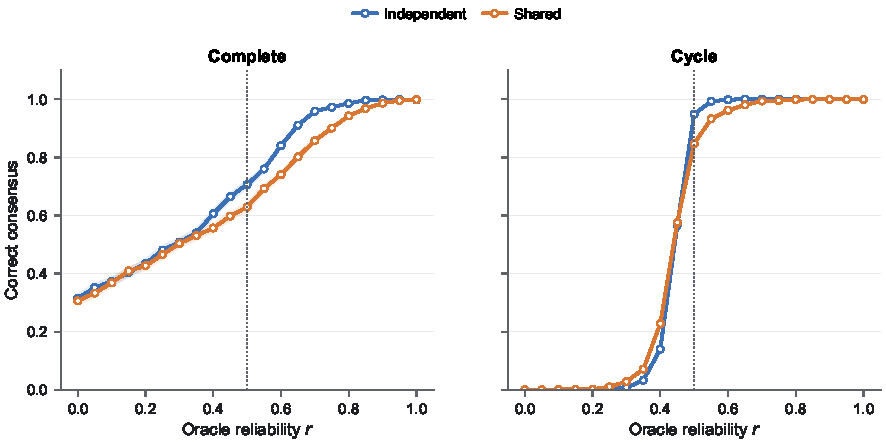
\includegraphics[width=0.86\textwidth]{figures/shared_vs_independent_testimony.pdf}
\caption{Correct-consensus probability under a common signal and independent
signals with the same marginal accuracy $r$, for complete and cycle networks at
$\varphi=1$. Vertical reference line at $r=0.5$. Each point aggregates $1000$
Monte Carlo runs; bands show one standard error.}
\label{fig:correlation}
\end{figure*}

\subsection{Community versus lone agent}

The same static source need not have the same consequences for a networked
community and for a lone agent. Figure~\ref{fig:individual} compares, across
$r$, (i)~a fully adopting community, (ii)~the same community with no source, and
(iii)~a single agent consulting the same static common source. On the cycle, a
shared biased source ($r\lesssim 0.4$) drives community correct-consensus rates
far below the no-source baseline and, over much of that region, below the
lone-agent rate under the identical source. On the complete graph, collective
harm relative to the no-source baseline is milder and confined to lower $r$, and
the community typically outperforms the lone agent. The comparison shows that
source accuracy alone does not determine whether consultation is collectively
beneficial: network structure and signal sharing mediate the gap between
individual and community outcomes.

\begin{figure*}[!t]
\centering
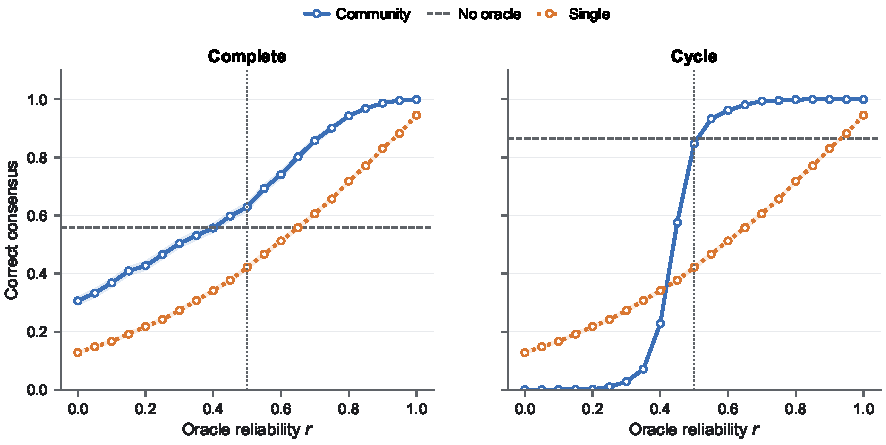
\includegraphics[width=0.86\textwidth]{figures/individual_help_collective_harm.pdf}
\caption{Correct-consensus probability for a fully adopting community, the
no-source community baseline, and a lone agent facing the same static source,
across source accuracy $r$. Community estimates use $1000$ seeds; lone-agent
estimates use $4000$ seeds.}
\label{fig:individual}
\end{figure*}

\section{Adaptive-Source and Topology Results}
\label{sec:adaptive}

\subsection{Adaptive versus static sources}

We compare three conditions at full adoption: no source, a static common source
with fixed accuracy $r=0.7$, and an adaptive source that updates from community
$b$-trials and rebroadcasts its posterior mean. Correct-consensus rates under
the adaptive source remain close to the no-source baseline on both topologies,
whereas the static $r=0.7$ source raises those rates substantially
(Fig.~\ref{fig:adaptive_rates}). On the cycle at $\varphi=1$, the adaptive
source is slightly below the no-source baseline in the displayed runs. The
comparison indicates that closing the feedback loop does not, in these settings,
reproduce the gains of a reliably accurate static source.

\begin{figure}[!t]
\centering
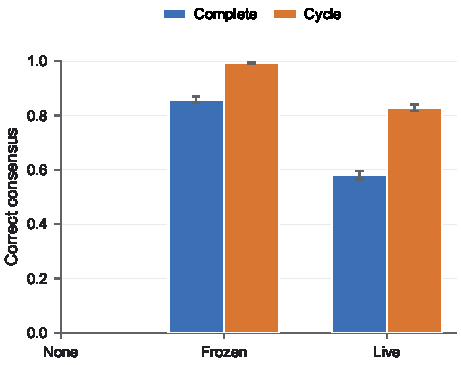
\includegraphics[width=0.96\columnwidth]{figures/adaptive_feedback_reliability.pdf}
\caption{Correct-consensus probability under no source, a static common source
with $r=0.7$, and an adaptive source that learns from community data, at
$\varphi=1$. Bars aggregate $1000$ Monte Carlo runs; error bars show one
standard error.}
\label{fig:adaptive_rates}
\end{figure}

\subsection{Conditional trajectories under the adaptive source}

We examine the fraction of agents choosing $b$ and the source posterior mean over
time on the complete graph with $\varphi=1$, separating trajectories by final
outcome. In runs ending in correct consensus, the fraction choosing $b$
approaches one. In runs ending in incorrect consensus, experimentation on $b$
approaches zero (Fig.~\ref{fig:exploration}). The source posterior separates
early across the two outcome groups and then changes little in incorrect runs
once $b$-trials disappear (Fig.~\ref{fig:sourcefreeze}).

\begin{figure}[!t]
\centering
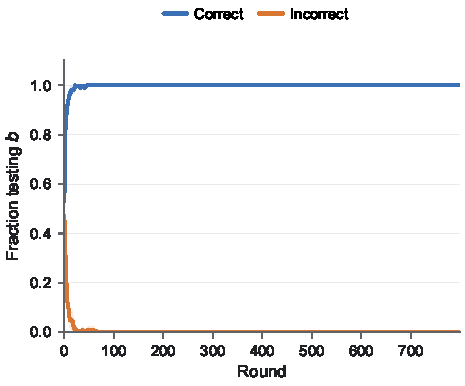
\includegraphics[width=0.96\columnwidth]{figures/better_arm_exploration.pdf}
\caption{Fraction of agents choosing the better action under the adaptive
source, with trajectories grouped by final outcome. Bands show means $\pm$ one
standard error across $300$ Monte Carlo runs on the complete graph at
$\varphi=1$.}
\label{fig:exploration}
\end{figure}

\begin{figure}[!t]
\centering
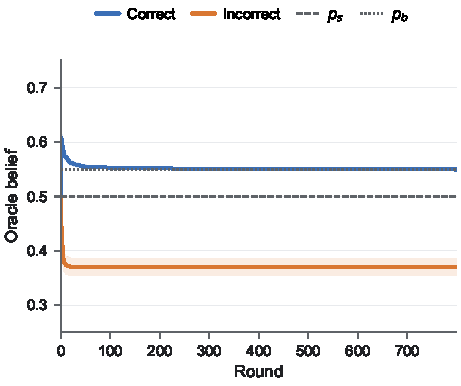
\includegraphics[width=0.96\columnwidth]{figures/adaptive_oracle_lock_in.pdf}
\caption{Adaptive-source posterior mean over time, with trajectories grouped by
final outcome. Horizontal references mark $p_s=0.5$ and $p_b=0.55$. When
experimentation on $b$ ends, the source receives no further data about $p_b$ and
its posterior stops changing.}
\label{fig:sourcefreeze}
\end{figure}

These trajectories identify a lock-in mechanism within the model. Source belief
affects later experimentation, and the cessation of experimentation prevents
further source learning. Together with Fig.~\ref{fig:adaptive_rates}, the
results show both that adaptive feedback can fail to improve on the no-source
baseline and how incorrect adaptive runs become informationally closed.

\subsection{Topology ranking across source accuracy}

The complete and cycle networks exchange rank as $r$ changes under a common
static source at $\varphi=1$ (Fig.~\ref{fig:inversion}). Under sufficiently
misleading common signals in the displayed settings, the complete network has a
higher correct-consensus rate than the cycle (for example, near $r=0.3$). At
higher source accuracy ($r\gtrsim 0.5$), the cycle performs better.

\begin{figure}[!t]
\centering
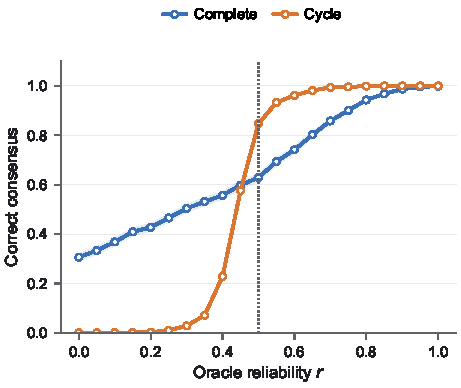
\includegraphics[width=0.96\columnwidth]{figures/network_structure_inversion.pdf}
\caption{Correct-consensus probability for complete and cycle networks across
source signal accuracy under a common static source at $\varphi=1$. The
intersection marks a ranking reversal between the two topologies under the
displayed parameter settings.}
\label{fig:inversion}
\end{figure}

A plausible explanation is that the source and the social network transmit
different kinds of information. A cycle can preserve heterogeneous responses to
local experimental evidence, but a common source reaches adopters without
traveling through the cycle's edges. Once a misleading common signal is present,
the cycle also transmits corrective experimental evidence more slowly. In a
complete graph, any corrective evidence generated by one agent is available to
all agents in the next update. Because complete and cycle graphs differ in
several structural properties, the comparison does not identify edge density
alone as the cause of the reversal.

\subsection{Robustness of the common-signal difference}

At $N=10$ and $r=0.6$, the independent-signal condition outperforms the
common-signal condition in all displayed combinations of $\varepsilon$ and
source influence $\tau$ (Fig.~\ref{fig:robustness}). The difference is larger
when source influence is high and often larger when the arm-quality gap is
small. Across the full robustness grid, including $N=20$, the estimated penalty
remains positive in every cell. The result establishes persistence across the
displayed neighborhood of the parameter space rather than universality.

\begin{figure}[!t]
\centering
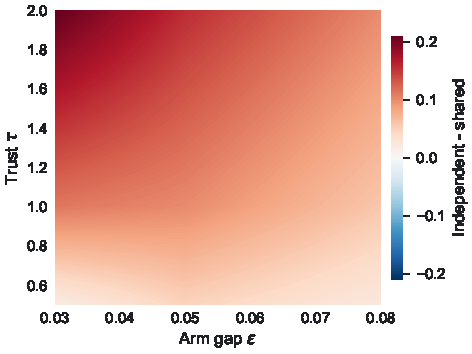
\includegraphics[width=0.94\columnwidth]{figures/correlation_penalty_robustness.pdf}
\caption{Difference in correct-consensus probability between independent and
common source signals at $N=10$ and $r=0.6$, across arm-quality gap
$\varepsilon$ and source influence $\tau$. Positive values favor independent
signals.}
\label{fig:robustness}
\end{figure}

\section{Adaptive Trust}
\label{sec:trust}

We next ask whether endogenous trust updating can mitigate a biased static
source. Adopters scale $\tau$ by an agreement-based moving average, with base
parameters $\varphi=0.7$ and $\tau=2$. Figure~\ref{fig:trust} compares fixed
trust with adaptive trust across source accuracy.

On the cycle, adaptive trust raises correct-consensus rates in a neighborhood of
moderately biased sources (near $r\approx 0.40$--$0.45$), where fixed trust
leaves the community well below its no-source baseline. On the complete graph,
gains under strong bias are smaller, and adaptive trust reduces correct-consensus
rates when the source is already reliable ($r\gtrsim 0.7$). The mechanism
therefore provides only partial protection: it can help where a biased common
source is most damaging on the cycle, but trust withdrawal is imperfect and can
discard useful testimony when the source is accurate.

\begin{figure*}[!t]
\centering
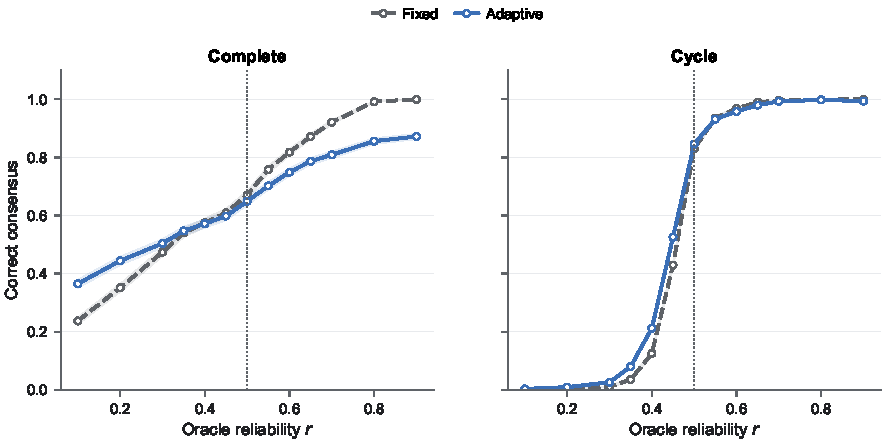
\includegraphics[width=0.86\textwidth]{figures/adaptive_trust_under_bias.pdf}
\caption{Correct-consensus probability under fixed versus adaptive trust in a
common static source, across source accuracy $r$, for complete and cycle
networks ($\varphi=0.7$, $\tau=2$). Vertical reference line at $r=0.5$. Each
point aggregates $1000$ Monte Carlo runs.}
\label{fig:trust}
\end{figure*}

\section{Discussion}
\label{sec:discussion}

\subsection{Signal dependence and collective learning}

The common-versus-independent comparison isolates the effect of dependence
among source signals. Each consultation has the same marginal probability of
favoring the better action in both conditions, but independent signals preserve
more variation across agents. Common signals instead move consulting agents in
the same direction within a round. When that direction is mistaken, the source
can reduce simultaneous experimentation on the better action across multiple
parts of the network.

This result is consistent with work on algorithmic monoculture and independent
information production \citep{kleinberg2021,heddenraghavan2026}. The present
model adds a separate social evidence-sharing network, making it possible to
study how source dependence interacts with the circulation of experimental
evidence. The community-versus-lone-agent comparison further shows that the same
source can be less damaging---or even relatively less harmful---for an isolated
decision maker than for a communicating community, especially under shared bias
on the cycle.

\subsection{Adaptive sources and endogenous evidence}

The adaptive-source comparisons show both an aggregate and a dynamic failure
mode. In aggregate, learning from community data does not yield the gains of a
fixed high-accuracy source and remains near the no-source baseline. Dynamically,
incorrect runs lose experimentation on $b$, after which the source's posterior
stops changing. The source changes agents' subsequent choices, those choices
determine which experiments are run, and the resulting evidence updates the
source. When agents stop testing the better action, both the community and the
source cease receiving information about it. An incorrect posterior can
therefore persist without further reinforcement simply because the relevant data
are no longer generated.

This mechanism differs from ordinary exposure to a fixed erroneous signal. The
source participates in the process that determines its future evidence. The
result is structurally related to performative prediction
\citep{perdomo2020}, although the outcome here is collective identification of a
superior action rather than predictive risk under a shifted data distribution.

\subsection{Network structure and the source environment}

The ranking reversal between complete and cycle networks shows that the effects
of communication structure depend on the source environment. Without an
external common signal, slower information transmission can preserve behavioral
variation and continued testing. With a misleading common signal, the same
slower transmission can impede the spread of corrective experimental evidence,
while the source reaches adopters independently of network distance.

The complete-versus-cycle comparison does not identify a single graph statistic
responsible for the reversal. The two networks differ in density, path length,
degree, and clustering. A fuller account would vary these properties separately
across larger graph families. The present result nevertheless establishes that
the relative performance of two standard network structures is not invariant to
the accuracy of a shared external source.

\subsection{Trust, implications, and scope}

Adaptive trust is a limited remedy in this model. It helps most where a biased
common source is especially harmful on the cycle, but it does not restore
no-source performance under strong bias, and it can reduce the value of reliable
sources on denser networks. Trust adjustment therefore does not eliminate the
collective risks identified above.

The model identifies several variables relevant to empirical studies of shared
decision-support systems: dependence among outputs, concentration of adoption,
the amount of independent experimentation remaining after adoption, whether
recommendations alter the data used for subsequent updating, and whether users
can revise trust fast enough to matter. The simulations do not determine the
prevalence or magnitude of these mechanisms in scientific, clinical,
journalistic, or public settings. Real systems may actively explore, use
heterogeneous data, provide user-specific outputs, and receive evidence that is
generated independently of user choices.

The model also abstracts from several features of real inquiry. It contains two
Bernoulli actions, Bayesian nonstrategic agents, homogeneous experimental
competence, and a source represented by a small set of parameters. Real
communities consider multiple hypotheses, differ in expertise and influence,
communicate strategically, and evaluate evidence of unequal quality. The static
source has exogenous accuracy, and the common signal is redrawn across rounds;
more persistent or state-dependent error processes may generate different
outcomes. Adoption is a fixed random fraction rather than endogenous selection
by network position or performance.

Results in this model family are sensitive to the payoff gap, prior strength,
number of trials per round, horizon, stopping rule, and network size
\citep{rosenstock2017}. The simulations therefore establish mechanisms and
comparative results under specified conditions rather than quantitative
predictions about AI adoption. Future work can test additional graph
families, persistent source errors, heterogeneous adoption positions, forced
exploration, alternative trust rules, alternative priors, and more than two
actions.

\section{Conclusion}
\label{sec:conclusion}

\balance
This study extends a standard epistemic-network model by adding an external
information source whose signal dependence can be varied independently of the
social communication network. In the simulations, common signals produce lower
correct-consensus rates than independent signals of equal marginal accuracy in
several parameter regions. The same shared source can harm a networked community
relative to a no-source baseline and, under bias on the cycle, relative to a lone
agent facing that source. An adaptive source that learns from community data
remains near the no-source baseline and far below a static high-accuracy source;
incorrect adaptive runs lose experimentation and freeze the source posterior.
Complete and cycle networks reverse their relative ranking as source accuracy
changes. Adaptive trust offers only partial mitigation. Collective learning in
this setting depends not only on source accuracy but also on the dependence
among source signals, the evidence agents continue to generate, trust
adjustment, and the network through which corrective evidence circulates.

\begin{thebibliography}{99}
\fontsize{8.1}{9.2}\selectfont

\bibitem[Bala and Goyal(1998)]{balagoyal1998}
Bala, V., \& Goyal, S. (1998). Learning from neighbours. \emph{Review of
Economic Studies}, 65(3), 595--621.

\bibitem[Banihashem et al.(2023)]{banihashem2023}
Banihashem, K., Hajiaghayi, M. T., Shin, S., \& Slivkins, A. (2023). Bandit
social learning under myopic behavior. In \emph{Advances in Neural Information
Processing Systems} (Vol. 36).

\bibitem[Bommasani et al.(2022)]{bommasani2022}
Bommasani, R., Creel, K. A., Kumar, A., Jurafsky, D., \& Liang, P. (2022).
Picking on the same person: Does algorithmic monoculture lead to outcome
homogenization? In \emph{Advances in Neural Information Processing Systems}
(Vol. 35, pp. 3663--3678).

\bibitem[Hedden and Raghavan(2026)]{heddenraghavan2026}
Hedden, B., \& Raghavan, M. (2026). Algorithmic monoculture and its critics.
\emph{arXiv preprint arXiv:2604.06047}.

\bibitem[Kleinberg and Raghavan(2021)]{kleinberg2021}
Kleinberg, J., \& Raghavan, M. (2021). Algorithmic monoculture and social
welfare. \emph{Proceedings of the National Academy of Sciences}, 118(22),
e2018340118. \url{https://doi.org/10.1073/pnas.2018340118}

\bibitem[O'Connor and Weatherall(2019)]{oconnor2019}
O'Connor, C., \& Weatherall, J. O. (2019). \emph{The Misinformation Age: How
False Beliefs Spread}. Yale University Press.

\bibitem[Perdomo et al.(2020)]{perdomo2020}
Perdomo, J. C., Zrnic, T., Mendler-D\"unner, C., \& Hardt, M. (2020).
Performative prediction. In \emph{Proceedings of the 37th International
Conference on Machine Learning} (Vol. 119, pp. 7599--7609). PMLR.

\bibitem[Rosenstock et al.(2017)]{rosenstock2017}
Rosenstock, S., Bruner, J., \& O'Connor, C. (2017). In epistemic networks, is
less really more? \emph{Philosophy of Science}, 84(2), 234--252.
\url{https://doi.org/10.1086/690717}

\bibitem[Weatherall et al.(2020)]{weatherall2020}
Weatherall, J. O., O'Connor, C., \& Bruner, J. P. (2020). How to beat science
and influence people: Policymakers and propaganda in epistemic networks.
\emph{The British Journal for the Philosophy of Science}, 71(4), 1157--1186.
\url{https://doi.org/10.1093/bjps/axy062}

\bibitem[Zollman(2007)]{zollman2007}
Zollman, K. J. S. (2007). The communication structure of epistemic communities.
\emph{Philosophy of Science}, 74(5), 574--587.

\bibitem[Zollman(2010)]{zollman2010}
Zollman, K. J. S. (2010). The epistemic benefit of transient diversity.
\emph{Erkenntnis}, 72(1), 17--35.

\end{thebibliography}

\end{document}
